\documentclass[12pt]{article}

\usepackage[dvips,letterpaper,margin=0.75in,bottom=0.75in]{geometry}
\usepackage{cite}
\usepackage{slashed}
\usepackage{graphicx}
\usepackage{amsmath}
\usepackage{braket}
\usepackage{latexsym,amssymb,amsmath}
\usepackage{pdfpages}
\usepackage{xcolor}


\usepackage[american,fulldiode]{circuitikz}
\tikzset{component/.style={draw,thick,circle,fill=white,minimum size =0.75cm,inner sep=0pt}}

\begin{document}
\ctikzset{bipoles/thickness=1}
\ctikzset{bipoles/length=.6cm}

\title{Overview of the Undergraduate Physics Curriculum}
\author{Michael Mulhearn}

\maketitle

\section{Objectives}

\section{Review of Preparatory Subject Matter}


A summary of the content in the core required courses:
\begin{itemize}

\item {\bf PHY 9A - Classical Physics (5)}
{\it Lecture—3 hours; laboratory—2.5 hours; discussion—1 hour. Prerequisite: Mathematics 21B. Introduction to general principles and analytical methods used in physics for physical science and engineering majors. Classical mechanics. Only 2 units of credit to students who have completed course 1A or 7B. Not open for credit to students who have completed course 9HA. GE credit: SciEng | SE. - III. (III.)}

\item {\bf PHY 9B - Classical Physics (5)}
{\it Lecture - 3 hours; laboratory - 2.5 hours; discussion - 1 hour. Prerequisite: course 9A [or 9HA], Mathematics 21C, 21D (may be taken concurrently). Continuation of course 9A. Fluid mechanics, thermodynamics, wave phenomena, optics. Only 2 units of credit to students who have completed course 7A. Not open for credit to students who have completed course 9HB, 9HC, or Engineering 105. - I. (I.)}

\item {\bf PHY 9C - Classical Physics (5)}
{\it Lecture - 3 hours; laboratory - 2.5 hours; discussion - 1 hour. Prerequisite; course 9B [or 9HC], Mathematics 21D, 22A (may be taken concurrently). Electricity and magnetism including circuits and Maxwell’s equations. Only 3 units of credit to students who have completed course 7C. Not open for credit to students who have completed course 9HD. GE credit: SciEng | SE. - II. (II.)}

\item {\bf PHY 9D - Modern Physics (4)}
{\it Lecture - 3 hours; discussion - 1.5 hours. Prerequisite: course 9C [or 9HD] and Mathematics 22A; Mathematics 22B recommended (may be taken concurrently). Introduction to physics concepts developed since 1900. Special relativity, quantum mechanics, atoms, molecules, condensed matter, nuclear and particle physics. Not open for credit to students who have completed course 9HB, 9HC, or 9HE. GE credit: SciEng | SE.- III. (III.)}

\item {\bf PHY 9HA - Honors Physics (5)}
{\it Lecture - 3 hours; discussion/laboratory - 4 hours. Prerequisite: Mathematics 21B (may be taken concurrently) or consent of instructor. Classical mechanics. Same material as course 9A in greater depth. For students in physical sciences, mathematics, and engineering. Only 2 units of credit to students who have completed course 7B. Not open for credit to students who have completed course 9A. GE credit: SciEng | SE. - I. (I.)}

\item {\bf 9HB - Honors Physics (5)}
{\it Lecture - 3 hours; discussion/laboratory - 4 hours. Prerequisite: Physics 9HA or 9A, Mathematics 21C (may be taken concurrently). Special relativity, thermal physics. Continuation of course 9HA. Only 2 units of credit to students who have completed course 7A. Not open for credit to students who have completed course 9B or 9D. GE credit: SciEng | SE. - II. (II.)}

\item {\bf 9HC - Honors Physics (5)}
{\it Lecture - 3 hours; discussion/laboratory - 4 hours. Prerequisite: course 9HB and Mathematics 21D (may be taken concurrently). Waves, sound, optics, quantum physics. Continuation of Physics 9HB. Only 2 units of credit to students who have completed course 7C. Not open for credit to students who have completed course 9B or 9D. GE credit: SciEng | SE.- III. (III.)
Recent Syllabi and More Complete Descriptions}

\item {\bf 9HD - Honors Physics (5)}
{\it Lecture - 3 hours; discussion/laboratory - 4 hours. Prerequisite: course 9HC and Mathematics 21D. Electricity and magnetism. Continuation of Physics 9HC. Not open for credit to students who have completed course 9C. GE credit: SciEng | SE. - I. (I.)}

\item {\bf 9HE - Honors Physics (5)}
{\it Lecture - 3 hours; discussion/laboratory - 4 hours. Prerequisite: course 9HD and Mathematics 22B (may be taken concurrently). Application of quantum mechanics. Not open for credit to students who have completed course 9D. GE credit: SciEng | SE. - II. (II.)}

\item {\bf PHY 40 — Introduction to Physics Computation (4)}
{\it Lecture—2 hour(s); Laboratory—4 hour(s). Introduction to programming using C++ with examples from computational physics. Introduction to modern tools used for scientific analysis, including Scientific computing with Python. GE credit: SE. Effective: 2018 Summer Session 2.}

\item {\bf PHY 80 — Experimental Techniques (4)}
{\it Lecture—2 hour(s); Laboratory—5 hour(s). Prerequisite(s): PHY 009D or PHY 009HD. Open to Physics and Applied Physics majors only. Experimental techniques. Design of circuits. Data analysis, sources of noise, statistical and systematic uncertainties. Light sources, detection, and measurement in basic optical systems. Effective: 2017 Fall Quarter.}

\end{itemize}

\section{Review of Core Subject Matter}

The present core required courses are:\\
\begin{tabular}{lllll}
& PHY 104A & 4 & Introductory Methods of Mathematical Physics \\
& PHY 105A & 4 & Analytical Mechanics\\
& (PHY 105B) & 4 & Analytical Mechanics\\
& PHY 110A & 4 & Electricity and Magnetism \\
& PHY 110B & 4 & Electricity and Magnetism  \\
& (PHY 110C) & 4 & Electricity and Magnetism  \\
& PHY 112   & 4 & Thermodynamics and Statistical Mechanics & 115A\\
& PHY 115A & 4 & Quantum Mechanics & 104A,105A\\
& PHY 115B & 4 & Quantum Mechanics & \\
\end{tabular}

Typical schedule for preparatory and core subject matter of 4 yr BS majors, omitting labs.

\begin{table}
\begin{center}
\begin{tabular}{|l|l|l|l|}
\hline
year      & fall    & winter & spring  \\
\hline
Freshman  & 9A/9HA  & 9B/9HB  & 9C/9HC \\
\hline
Sophomore & 9D/9HD  & (9HE)   & 40     \\
          &         &         &        \\
\hline
Junior    & 104A & 105B & 110B\\
          & 105A & 110A & 115A\\
\hline
Senior    & 115B &        & \\
          & 110C &        & \\
          & 112  &        & \\

\hline 
\end{tabular}
\end{center}
\end{table}
For Junior transfers the typical schedule omitting labs is:
\begin{table}
\begin{center}
\begin{tabular}{|l|l|l|l|}
\hline
year      & fall    & winter & spring  \\
\hline
Junior    & 9D  &    & 40     \\
          & 104A & 105B & 110B\\
          & 105A & 110A & 115A\\
          & 102 &       & \\

\hline
Senior    & 115B &        & \\
          & 112  &        & \\

\hline 
\end{tabular}
\end{center}
\end{table}
 



A summary of the content in the core required courses:
\begin{itemize}
\item {\bf PHY 104A - Introductory Methods of Mathematical Physics}
{\it Lecture - 3 hours; extensive problem solving. Prerequisite: courses 9B, 9C, 9D [or 9HB, 9HC, 9HD] and Mathematics 21D, 22A, and 22B with grade C- or better or consent of instructor. Introduction to the mathematics used in upper-division physics courses, including applications of vector spaces, Fourier analysis, partial differential equations. - I. (I.)}

Recently taught by Scalettar and Luty.  Luty teaches this as a boot camp for upper division courses:  vectors, expansion in small parameters, and PDEs.  All topics which are in principle should have been seen before, but students clearly need practice with problems.

\item {\bf PHY 105A - Analytical Mechanics}
{\it Lecture - 3 hours; extensive problem solving. Prerequisite: courses 9B, 9C, 9D [or 9HB, 9HC, 9HD] and Mathematics 21D, 22A, and 22B passed with grade C– or better; or consent of department; course 104A and 105A passed with a grade C– or better or consent of department required for 105B. Principles and applications of Newtonian mechanics; introduction to Lagrange’s and Hamilton’s equations. - I-II. (I-II.)}

Recently taught by Calderon, Cebra, Svoboda, and Conway.  Covers Morin 1-5.  This course is heavy on problem solving.  Morin focuses more on challenging problems, and less on mathematical formalism (e.g. leaves out Hamiltonian)
Not all instructors reach 5 in first quarter.

\item {\bf PHY 105B - Analytical Mechanics}
{\it Lecture - 3 hours; extensive problem solving. Prerequisite: courses 9B, 9C, 9D [or 9HB, 9HC, 9HD] and Mathematics 21D, 22A, and 22B passed with grade C– or better; or consent of department; course 104A and 105A passed with a grade C– or better or consent of department required for 105B. Principles and applications of Newtonian mechanics; introduction to Lagrange’s and Hamilton’s equations. - I-II. (I-II.)}

Recently taught by Pickett, Conway.  Covers Morin 6-11.  Picket supplement chapter 5 with supplemental material for Hamiltonian.

\item {\bf PHY 110A - Electricity and Magnetism}
{\it Lecture - 3 hours; extensive problem solving. Prerequisite: courses 9B, 9C, 9D [or 9HB, 9HC, 9HD] and Mathematics 21D, 22A, and 22B passed with grade C– or better, or consent of department; prerequisite for 110B is courses 110A and 104A passed with a grade of C– or better or consent of department; prerequisite for course 110C is courses 110B and 104B passed with a grade of C– or better, or consent of department. Theory of electrostatics, electromagnetism, Maxwell’s equations, electromagnetic waves. - II-III-I. (II-III-I.)}

Recently taught by Da Silva Neto and Yu.  Covers Griffiths 1-4.  Yu extends to include complex analysis of La Place's equation.  Includes a recap of vector calculus, but Da Silva Neto reports a benefit from 104A  (Math Methods.)

\item {\bf PHY 110B - Electricity and Magnetism}
{\it Lecture - 3 hours; extensive problem solving. Prerequisite: courses 9B, 9C, 9D [or 9HB, 9HC, 9HD] and Mathematics 21D, 22A, and 22B passed with grade C– or better, or consent of department; prerequisite for 110B is courses 110A and 104A passed with a grade of C– or better or consent of department; prerequisite for course 110C is courses 110B and 104B passed with a grade of C– or better, or consent of department. Theory of electrostatics, electromagnetism, Maxwell’s equations, electromagnetic waves. - II-III-I. (II-III-I.)}

Recently taught by Yu.  Griffiths 5-9.  Rapid pace for subject matter, so problem solving is left mainly for homework.  No breathing room for computational physics.

\item {\bf PHY 110C - Electricity and Magnetism}
{\it Lecture - 3 hours; extensive problem solving. Prerequisite: courses 9B, 9C, 9D [or 9HB, 9HC, 9HD] and Mathematics 21D, 22A, and 22B passed with grade C– or better, or consent of department; prerequisite for 110B is courses 110A and 104A passed with a grade of C– or better or consent of department; prerequisite for course 110C is courses 110B and 104B passed with a grade of C– or better, or consent of department. Theory of electrostatics, electromagnetism, Maxwell’s equations, electromagnetic waves. - II-III-I. (II-III-I.)}

Recently taught by Yu and Luty.  Rest of Griffiths.   Potentials (including vector potential), radiation in matter, special relativity.

\item {\bf PHY 112 - Thermodynamics and Statistical Mechanics}
{\it Lecture - 3 hours; extensive problem solving. Prerequisite: course 115A or the equivalent. Introduction to classical and quantum statistical mechanics and their connections with thermodynamics. The theory is developed for the ideal gas model and simple magnetic models and then extended to studies of solids, quantum fluids, and chemical equilibria. - I. (I.)}

Recently taught by Singh, Da Silva Neto.  Based on Shroeder.  
Fast review of 1 (Thermodynamics), full coverage of 2 and 3 (Entropy/Temperature starting from quantum systems up to ideal gas) skip 4 (Heat engines), Free energy part of 5, full coverage of 6+7 (Boltzman and Quantum statistics).

\item {\bf PHY 115A - Foundation of Quantum Mechanics}
{\it Lecture - 3 hours; extensive problem solving. Prerequisite: courses 104A and 105A with grade C- of better, or consent of instructor. Introduction to the methods of quantum mechanics with applications to atomic, molecular, solid state, nuclear and elementary particle physics. - III. (III.)} 

Recently taught by Fong,Curro.  Townsend for undergraduate version of Sakurai's spin-first approach.  Chapters 1-5, sometimes 6.

\item {\bf PHY 115B - Applications of Quantum Mechanics}
{\it Lecture - 3 hours; extensive problem solving. Prerequisite: course 115A passed with a grade of C– of better, or consent of department. Angular momentum and spin; hydrogen atom and atomic spectra; perturbation theory; scattering theory. - I. (I.)}

Recently taught by Curro.  Townsend 6,7, skip 8 (path integrals), then 9-10.
Leaves off perturbation theory, identical particles, scattering.

\end{itemize}


\section{Objectives}

\section{Open Questions}
\begin{itemize}
\item What is the role of advanced classes not part of any major or specialization:  104C,123,...  Is 105C ever offered?  It seems required for physical oceanography.
\item What actually is the maximum number of required credits allowed in a major?
Looks empirically like 90 for some reason...
\end{itemize}

\section{Answered Questions}
\begin{itemize}
\item Can we require a class if e.g. less than A in certain prerequisites? No.  C- is threshold for pre-req.
\item Do specializations have to stay within any credit limits?  Could we have "Physics BS with specialization in Computational Physics" that exceeds credit limits?  No.
\item Astrophysics specializations comes at high extra course load:  180,150-156, and lab course 157.  Is this "fair" to the non-astro faculty?  Can this foot print be reduced?  For elective courses, students vote with their feet, and Astronomy electives are popular.  Labs have been discontinued and many of these courses are offered only every other year. 
\end{itemize}


\section{Problems and Ideas}
\begin{itemize}
\item Relevant stuff for QM (Angular Momentum, Central Forces) is in 105B, but only 105A is a preq.  In general, 105B is major absence from applied physics requirements.  Not all 105A+B instructors even cover Hamiltonian formalism.
\item 104A is taught by Luty as a sort of boot camp for problem solving in upper division courses... but only a pre-req for 115A.
\item Damped driven oscillator is missing from mechanics.
\item We don't always cover Hamiltonian formalism before reaching QM.
\item Drop 110C.  Need to cover vector potential in B.  Need to cover special relativity elsewhere.
\item Curro thinks we need to add QIT somewhere, at least as elective, or risk being left behind.
\end{itemize}

\section{Big Ideas}
\begin{itemize}
\item We have three tracks, essentially:  9H, 9, and transfers.  Current policy amounts to asking 9H students to wait for everyone else.  Maybe we can make 9H students overlap other tracks in Sophomore (vs Junior) year.
\item More computing!!!
\end{itemize}

\newpage

\includepdf[pages=1,pagecommand={\begin{tikzpicture}[remember picture, overlay]
    \end{tikzpicture}}]{tocs/morin_toc.pdf}

\includepdf[pages=3,pagecommand={\begin{tikzpicture}[remember picture, overlay]
      \node[left] at (0.25, -7.5) {\color{red} 105A};
      \node[left] at (0.25, -10.3) {\color{red} 105A};
      \node[left] at (0.25, -15) {\color{red} 105A};
      \node[left] at (0.25, -20.2) {\color{red} 105A};
    \end{tikzpicture}}]{tocs/morin_toc.pdf}

\includepdf[pages=4,pagecommand={\begin{tikzpicture}[remember picture, overlay]
      \node[left] at (0.25, -9.5) {\color{red} 105A/B};
      \node[left] at (0.25, -17) {\color{red} 105B};
    \end{tikzpicture}}]{tocs/morin_toc.pdf}

\includepdf[pages=5,pagecommand={\begin{tikzpicture}[remember picture, overlay]
      \node[left] at (0.25, -2.3) {\color{red} 105B};
      \node[left] at (0.25, -11.3) {\color{red} 105B};
    \end{tikzpicture}}]{tocs/morin_toc.pdf}

\includepdf[pages=6,pagecommand={\begin{tikzpicture}[remember picture, overlay]
      \node[left] at (0.25, -2.3) {\color{red} 105B};
      \node[left] at (0.25, -7.7) {\color{red} 105B};
      \node[left] at (0.25, -17.8) {\color{red} 105B};
    \end{tikzpicture}}]{tocs/morin_toc.pdf}

\includepdf[pages=7,pagecommand={\begin{tikzpicture}[remember picture, overlay]
    \end{tikzpicture}}]{tocs/morin_toc.pdf}

\includepdf[pages=8,pagecommand={\begin{tikzpicture}[remember picture, overlay]
    \end{tikzpicture}}]{tocs/morin_toc.pdf}


\includepdf[pages=1,pagecommand={\begin{tikzpicture}[remember picture, overlay]
    \end{tikzpicture}}]{tocs/griffiths_toc.pdf}

\includepdf[pages=6,pagecommand={\begin{tikzpicture}[remember picture, overlay]
      \node[left] at (0.25, -7.4) {\color{red} 110A};
    \end{tikzpicture}}]{tocs/griffiths_toc.pdf}

\includepdf[pages=7,pagecommand={\begin{tikzpicture}[remember picture, overlay]
      \node[left] at (0.25, -2.8) {\color{red} 110A};
      \node[left] at (0.25, -17.8) {\color{red} 110A};
    \end{tikzpicture}}]{tocs/griffiths_toc.pdf}

\includepdf[pages=8,pagecommand={\begin{tikzpicture}[remember picture, overlay]
      \node[left] at (0.25, -7.8) {\color{red} 110A};
      \node[left] at (0.25, -18.4) {\color{red} 110B};
    \end{tikzpicture}}]{tocs/griffiths_toc.pdf}

\includepdf[pages=9,pagecommand={\begin{tikzpicture}[remember picture, overlay]
      \node[left] at (0.25, -5.7) {\color{red} 110B};
      \node[left] at (0.25, -15.2) {\color{red} 110B};
    \end{tikzpicture}}]{tocs/griffiths_toc.pdf}

\includepdf[pages=10,pagecommand={\begin{tikzpicture}[remember picture, overlay]
      \node[left] at (0.25, -2.5) {\color{red} 110B};
      \node[left] at (0.25, -8.5) {\color{red} 110B};
      \node[left] at (0.25, -20.6) {\color{red} 110C};
    \end{tikzpicture}}]{tocs/griffiths_toc.pdf}

\includepdf[pages=11,pagecommand={\begin{tikzpicture}[remember picture, overlay]
      \node[left] at (0.25, -5.2) {\color{red} 110C};
      \node[left] at (0.25, -11.6) {\color{red} 110C};
    \end{tikzpicture}}]{tocs/griffiths_toc.pdf}

\includepdf[pages=12,pagecommand={\begin{tikzpicture}[remember picture, overlay]
    \end{tikzpicture}}]{tocs/griffiths_toc.pdf}

\includepdf[pages=1,pagecommand={\begin{tikzpicture}[remember picture, overlay]
    \end{tikzpicture}}]{tocs/townsend_toc.pdf}

\includepdf[pages=3,pagecommand={\begin{tikzpicture}[remember picture, overlay]
      \node[left] at (0.25, -6.2) {\color{red} 115A};
      \node[left] at (0.25, -11.2) {\color{red} 115A};
      \node[left] at (0.25, -17.5) {\color{red} 115A};
    \end{tikzpicture}}]{tocs/townsend_toc.pdf}

\includepdf[pages=4,pagecommand={\begin{tikzpicture}[remember picture, overlay]
      \node[left] at (0.25, -0.3) {\color{red} 115A};
      \node[left] at (0.25, -6) {\color{red} 115A};
      \node[left] at (0.25, -12) {\color{red} 115A/B};
      \node[left] at (0.25, -20.2) {\color{red} 115B};
    \end{tikzpicture}}]{tocs/townsend_toc.pdf}

\includepdf[pages=5,pagecommand={\begin{tikzpicture}[remember picture, overlay]
      \node[left] at (0.25, -13.5) {\color{red} 115B};
    \end{tikzpicture}}]{tocs/townsend_toc.pdf}

\includepdf[pages=6,pagecommand={\begin{tikzpicture}[remember picture, overlay]
      \node[left] at (0.25, -0.5) {\color{red} 115B};
    \end{tikzpicture}}]{tocs/townsend_toc.pdf}

\includepdf[pages=7,pagecommand={\begin{tikzpicture}[remember picture, overlay]
    \end{tikzpicture}}]{tocs/townsend_toc.pdf}

\begin{center}
   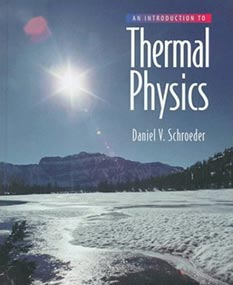
\includegraphics[scale=2.2]{tocs/schroeder_cover.jpg}
\end{center}

\includepdf[pages=1,pagecommand={\begin{tikzpicture}[remember picture, overlay]
    \node[left] at (0.25, -9.7) {\color{red} 112};
    \node[left] at (0.25, -16.7) {\color{red} 112};
    \end{tikzpicture}}]{tocs/schroeder_toc.pdf}

\includepdf[pages=2,pagecommand={\begin{tikzpicture}[remember picture, overlay]
    \node[left] at (0.25, 0.1) {\color{red} 112};
    \node[left] at (0.25, -13.2) {\color{red} 112};
    \node[left] at (2.2, -13.8) {\color{red} (Free Energy Only)};
    \end{tikzpicture}}]{tocs/schroeder_toc.pdf}

\includepdf[pages=3,pagecommand={\begin{tikzpicture}[remember picture, overlay]
    \node[left] at (0.25, -1.5) {\color{red} 112};
    \node[left] at (0.25, -7.7) {\color{red} 112};
    \end{tikzpicture}}]{tocs/schroeder_toc.pdf}

\includepdf[pages=4,pagecommand={\begin{tikzpicture}[remember picture, overlay]
    \end{tikzpicture}}]{tocs/schroeder_toc.pdf}


\end{document}






Upper Division Courses
102. Computational Laboratory in Physics (1)
Laboratory - 3 hours. Prerequisite: Mathematics 21D, 22A, 22B, Computer Science Engineering 30, course 9D or 9HD, course 104A concurrently. Introduction to computational physics and to the computational resources in the physics department. Preparation for brief programming assignments required in other upper division physics classes. Not open for credit to students who have completed course 104B or 105AL. - I. (I.) Fong
Recent Syllabus and More Complete Descriptions



104B. Computational Methods of Mathematical Physics (4)
Lecture - 3 hours; extensive problem solving. Prerequisite: course 104A with grade C- or better and course 105AL or consent of instructor. Introduction to the use of computational techniques to solve the mathematical problems that arise in advanced physics courses, complementing the analytical approaches emphasized in course 104A. - II. (II.)
Recent Syllabi and More Complete Descriptions












NON-CORE:
Advanced and Specialty Classes:

104C. Intermediate Methods of Mathematical Physics (4)
Lecture - 3 hours; extensive problem solving. Prerequisite: course 104A with grade C- or better or consent of instructor. Applications of complex analysis, conditional probability, integral transformations and other advanced topics. Not offered every year.
Recent Syllabi and More Complete Descriptions

105C. Continuum Mechanics (4)
Lecture - 3 hours; extensive problem solving. Prerequisite: courses 104B and 105A passed with a grade of C– or better, or consent of department. The continuum hypothesis and limitations. Tensor methods develop stress-strain relations for linear isotropic solids/fluids and field equations to study wave propagation in solids/fluids, heat flow, potential flow and ocean waves. - III. (III.)

108. Optics (3)
Lecture - 3 hours. Prerequisite: course 9 [or 9H] or 7 sequence and Mathematics 21 sequence or consent of instructor. The phenomena of diffraction, interference, and polarization of light, with applications to current problems in astrophysics, material science, and atmospheric science. Study of modern optical instrumentation. Open to non-majors. - III. (III.) Recent Syllabi and More Complete Descriptions

108L. Optics Laboratory (1)
Laboratory - 3 hours. Prerequisite: course 108 concurrently. The laboratory will consist of one major project pursued throughout the quarter, based on modern applications of optical techniques. - III. (III.)



116A. Electronic Instrumentation (4)
Lecture - 3 hours; laboratory - 3 hours. Prerequisite: course 9C [or 9HD], Mathematics 22B. An experimental and theoretical study of important electronic circuits commonly used in physics. - I. (I.)
Recent Syllabi and More Complete Descriptions

116B. Electronic Instrumentation (4)
Lecture - 3 hours; laboratory - 3 hours. Prerequisite: courses 9D [or 9HD], 116A. Continuation of course 116A. Introduction to the use of digital electronics and microcomputers in experimental physics. - II. (II.)
Recent Syllabi and More Complete Descriptions

116C. Introduction to Computer-Based Experiments in Physics (4)
Lecture - 3 hours; laboratory - 3 hours. Prerequisite: course 9D or 9HD, 116B, Mathematics 22B or consent of instructor. Introduction to techniques for making physical measurements using computer-based instrumentation. - III. (III.) Pellett
Recent Syllabi and More Complete Descriptions

122A. Advanced Physics Laboratory in Condensed Matter Physics (4) (Formerly Physics 122) 
Laboratory - 8 hours. Prerequisite: course 104A, 105A, 110B, and 112 (may be taken concurrently) or consent of the department, course 115A with grade of C- or better or consent of department. Experimental techniques and measurements in solid-state physics. Student performs three to six experiments depending on difficulty. Individual work is stressed. Thorough write-ups of the experiments are required. - II. (II.)
Recent Syllabus and More Complete Descriptions

122B. Advanced Physics Laboratory in Particle Physics (4) (Formerly Physics 122) 
Laboratory - 8 hours. Prerequisite: course 104A, 105A, 110B, and 112 (may be taken concurrently) or consent of the department, course 115A with grade of C- or better or consent of department. Experimental techniques and measurements in nuclear and particle physics. Student performs three to six experiments depending on difficulty. Individual work is stressed. Thorough write-ups of the experiments are required. - II. (II.)
Recent Syllabus and More Complete Descriptions

123. Signals and Noise in Physics (4) 
Lecture - 3 hours; extensive problem solving. Prerequisite(s): Physics 9ABCD [or 9HA-9HD] and 104A, or consent of instructor. Techniques of measurement and analysis designed to avoid systematic error and maximize signal/noise ratio. Illustrative examples of optimal filters ranging from condensed matter to cosmology. - II. (II.)
Recent Syllabus
Recent Flyer

129A. Introduction to Nuclear Physics (4) 
Lecture - 3 hours; extensive problem solving. Prerequisite: course 115A passed with a grade of C- or better or consent of instructor. Survey of basic nuclear properties and concepts requiring introductory knowledge of quantum mechanics: nuclear models and forces, radioactive decay and detecting nuclear radiation and nuclear reaction products, alpha, beta and gamma decay. - III. (III.)
Recent Syllabus and More Complete Descriptions

130A-130B. Elementary Particle Physics (4-4)
Lecture - 3 hours; extensive problem solving. Prerequisite: course 115A passed with a grade of C- or better or consent of instructor. Properties and classification of elementary particles and their interactions. Experimental techniques. Conservation laws and symmetries. Strong, electromagnetic, and weak interactions. Introduction to Feynman calculus. - II-III. (II-III.)
Recent Syllabi and More Complete Descriptions

140A-140B. Introduction to Solid State Physics (4-4)
Lecture - 3 hours; extensive problem solving. Prerequisite: course 115A or the equivalent passed with a grade of C- or better or consent of instructor. Survey of fundamental ideas in the physics of solids, with selected device applications. Crystal structure, x-ray and neutron diffraction, phonons, simple metals, energy bands and Fermi surfaces, semiconductors, optical properties, magnetism, superconductivity. - II-III. (II-III.)
Recent Syllabus 140A, Recent Syllabus 140B

150. Special Topics in Physics (4)
Lecture - 3 hours; extensive problem solving. Prerequisite(s): Physics 9ABCD or 9HA, HB, HC, HD, HE or consent of instructor. Topics vary, covering areas of contemporary research in physics. - I-II-III. (I-II-III.) Offered irregularly/on demand.

151. Stellar Structure and Evolution (4)
Lecture - 3 hours; extensive problem solving. Prerequisite(s): Physics 9ABCD [or 9HA-9HE] or consent of instructor. The chemical composition, structure, energy sources and evolutionary history of stars, with equal emphasis on both the observational data and theoretical models, including black holes, neutron stars and white dwarfs and the formation of substellar masses. - I. (I.) Not offered every year.
Recent Syllabus

152. Galactic Structure and the Interstellar Medium (4)
Lecture - 3 hours; extensive problem solving. Prerequisite(s): Physics 9ABCD [or 9HA-9HE] and Physics 105A concurrently or consent of instructor. The structure, contents, and formation of our Milky Way galaxy, viz. its shape and size, the nature of the interstellar medium, stellar populations, rotation curves, mass determination and evidence of dark matter. - I. (I.) Not offered every year.
Recent Syllabus

153. Extragalactic Astrophysics (4)
Lecture - 3 hours; extensive problem solving. Prerequisite(s): Physics 9ABCD [or 9HA-9HE] and Physics 104A and 105A or consent of the instructor.Not open to students who have taken Physics 127. Structure and evolution of galaxies and clusters of galaxies, including distance and mass determination, galaxy types and environments, active galactic nuclei and quasars, gravitational lensing and dark matter, global cosmological properties. - II. (II.) Not offered every year.
Recent Syllabus

154. Astrophysical Applications of Physics (4)
Lecture - 3 hours; extensive problem solving. Prerequisite(s): Physics 105AB, 110A; 110B, and 115A concurrently; 112 or consent of instructor. Not open to students who have taken this course previously as Physics 198. Applications of classical and quantum mechanics, thermodynamics, statistical mechanics, and electricity and magnetism to astrophysical settings such as the Big Bang, degenerate white dwarf and neutron stars, and solar neutrinos. - III. (III.) Not offered every year.

155. General Relativity (4)
Lecture - 3 hours; extensive problem solving. Prerequisite(s): Physics 104A and 105A; 105B and 110A or consent of instructor. Definition of the mathematical frame work for the description of the gravitational field, introduction of the dynamical equations of Einstein governing its evolution and review of the key solutions, including black holes and expanding universes. - II. (II.) Not offered every year.
Recent Syllabus

156. Introduction to Cosmology
Lecture - 3 hours; extensive problem solving. Prerequisite(s): Physics 9ABCD [or 9HA-9HE] and Physics 105A or consent of instructor. Not open to students who have taken Physics 126. Contemporary knowledge regarding the origin of the universe, including the Big Bang and nucleosynthesis, microwave background radiation, formation of cosmic structure, cosmic inflation, cosmic acceleration and dark energy. - II. (II.) Not offered every year.

157. Astronomy Instrumentation and Data Analysis Laboratory
Lecture - 2 hours; laboratory - 6 hours; extensive problem solving. Prerequisite(s): Physics 9ABCD [or 9HA-9HE]. Experimental techniques, data acquisition and analysis involving stellar, nebular and galaxy digital imaging, photometry and spectroscopy. Analyzing time resolved changes in the solar atmosphere in the light of hydrogen alpha. - III. (III.) Not offered every year.
Recent Syllabus

160. Environmental Physics and Society (3)
Lecture - 3 hours. Prerequisite: course 9D [or 9HD] or 7C; or course 10 or 1B and Mathematics 16B or the equivalent. Impact of humankind on the environment will be discussed from the point of view of the physical sciences. Calculations based on physical principles will be made, and the resulting policy implications will be considered. (Same course as Engineering 160.) GE credit: SciEng or SocSci. - III. (III.)

185. Careers in Physics (1)
Seminar - 1 hour. Designed to give Physics graduate students an in-depth appreciation of career opportunities with a graduate degree in physics. Professional physicists, mainly from outside academia, will give seminars describing both research and career insights. - II. (II.)
Recent Syllabi and More Complete Descriptions

190. Careers in Physics (1)
Seminar - 2 hours. Overview of important research areas in physics, discussions of research opportunities and internships, strategies for graduate school and industrial careers, the fellowship and assistantship selection process, preparation of resumes, personal statements, and letters of recommendation. - I. (I.)
Recent Syllabus

194HA-194HB. Special Study for Honors Students (4-4)
Independent study - 12 hours. Prerequisite: consent of instructor required. Open only to Physics and Applied Physics majors who satisfy the College of Letters and Science requirements for entrance into the Honors Program. Independent research project at a level significantly beyond that defined by the normal physics curriculum. (Deferred grading only, pending completion of sequence).

195. Senior Thesis (5)
Independent study - 15 hours. Prerequisite: consent of instructor required. Open only to Physics and Applied Physics majors with senior standing. Preparation of a senior thesis on a topic selected by the student with approval of the department. May be repeated for a total of 15 units. - I-II- III. (I-II-III.)

197T. Tutoring in Physics and Astronomy (1-5)
Tutoring of students in lower division courses. Leading of small voluntary discussion groups affiliated with one of the department’s regular courses. Weekly meeting with instructor. (P/NP grading only.) - I-II-III. (I-II-III.)

198. Directed Group Study (1-5)
Prerequisite: consent of instructor. (P/NP grading only.)
Recent Syllabi and More Complete Descriptions

199. Special Study for Advanced Undergraduates (1-5)
(P/NP grading only.)




\end{document}
